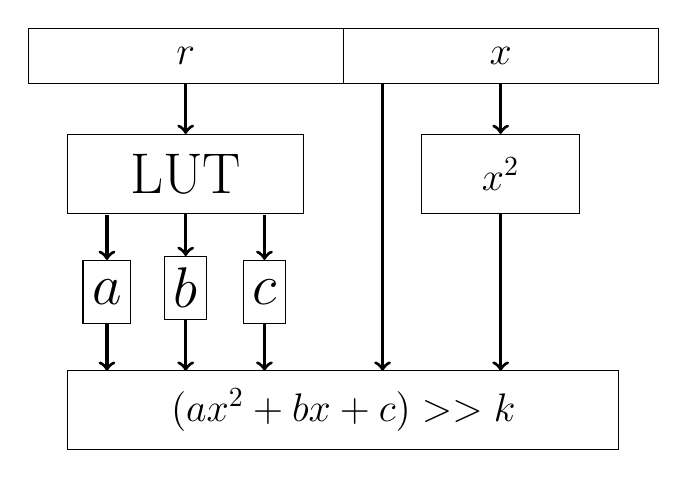
\begin{tikzpicture}

%draw input nodes
\node [shape=rectangle,draw = black, minimum width = 4cm,minimum height=0.7cm] at (0,6.5) (r) {\Large $r$};
% \node [shape=rectangle,draw = black, minimum width = 1cm,minimum height=0.7cm] at (2.5,6.5) (x_top) {\Large $s$};
\node [shape=rectangle,draw = black, minimum width = 4cm,minimum height=0.7cm] at (4,6.5) (x) {\Large $x$};

%draw lookup table with nodes output from LUT
\node [shape=rectangle,draw = black, minimum width = 3cm,minimum height=1cm] at (0,5) (lut) {\huge LUT};
\node [shape=rectangle,draw=black, minimum height = 0.8cm] at (-1,3.5) (a) {\huge $a$};
\node [shape=rectangle,draw=black, minimum height = 0.8cm] at (0,3.55) (b) {\huge $b$};
\node [shape=rectangle,draw=black, minimum height = 0.8cm] at (1,3.5)  (c) {\huge $c$};

\node [shape=rectangle,draw = black,minimum height=1cm, minimum width = 2cm] at (4,5) (square) {\Large$x^2$};
% \node[isosceles triangle, draw=black, rotate=270, minimum size =0.5cm] (invert) at (2.5,5.5){};

% \draw[] (2.5,5) circle (0.05);
% \node (invert_tip) at (2.5,5.05){};

%draw output box
\node [shape=rectangle,draw = black,minimum height=1cm, minimum width = 7cm] at (2,2) (poly) {\Large{$(ax^2+bx+c) >>k$}};

\node[] (left_x) at (2.5,6.28) {};
\draw [->,very thick] (left_x) edge (2.5,2.5);
% \draw [->,very thick] (invert_tip) edge (2.5,2);
\draw [->,very thick] (x) edge (square);
%Lines between input and LUT or final output box
\draw [->,very thick] (r) edge (lut);
% \draw [very thick] (2.5,4.5) edge (4.75,4.5);


\node[] (left_lut) at (-1,4.6) {};
\node[] (right_lut) at (1,4.6) {};
%Edges between LUT and outcomes
\draw [->,very thick] (left_lut) edge (a);
\draw [->,very thick] (lut) edge (b);
\draw [->,very thick] (right_lut) edge (c);

\draw [->,very thick] (a) edge (-1,2.5);
\draw [->,very thick] (b) edge (0,2.5);
\draw [->,very thick] (c) edge (1,2.5);

\draw [->,very thick] (square) edge (4,2.5);
\end{tikzpicture}